\documentclass[11pt, a4paper]{article}

\usepackage[czech]{babel}
\usepackage[utf8]{inputenc}
\usepackage[T1]{fontenc}
\usepackage{times}
\usepackage[left=2cm, top=3cm, text={17cm, 24cm}]{geometry}
\usepackage[unicode, colorlinks, hypertexnames=false, citecolor=red]{hyperref}
\usepackage{tabto}
\hypersetup{colorlinks = true, hypertexnames = false}
\usepackage{graphicx} 
\usepackage{listings}
\usepackage{color}
%\usepackage[outdir=./]{epstopdf}

\definecolor{dkgreen}{rgb}{0,0.6,0}
\definecolor{gray}{rgb}{0.5,0.5,0.5}
\definecolor{mauve}{rgb}{0.58,0,0.82}

\lstset{language=C,
  aboveskip=3mm,
  belowskip=3mm,
  showstringspaces=false,
  columns=flexible,
  basicstyle={\small\ttfamily},
  numbers=none,
  numberstyle=\tiny\color{gray},
  keywordstyle=\color{blue},
  commentstyle=\color{dkgreen},
  stringstyle=\color{mauve},
  breaklines=true,
  breakatwhitespace=true,
  tabsize=3,
  inputencoding=utf8,
  extendedchars=true,
  literate={á}{{\'a}}1 {ú}{{\'a}}1 {é}{{\'e}}1 {í}{{\'i}}1   {ý}{{\'y}}1 {č}{{\v{c}}}1 {ť}{{\'t}}1 {ľ}{{\'l}}1 
}

\begin{document}
	\begin{titlepage}
		\begin{center}
			\Huge
			\textsc{Vysoké učení technické v~Brně} \\
			\huge
			\textsc{Fakulta informačních technologií} \\
			\vspace{\stretch{0.382}}
			\LARGE
			Projektová dokumentácia k~predmetu ISA \\
			\Huge
			Monitoring SSL spojenia
			\vspace{\stretch{0.618}}
		\end{center}

		{\Large
			\today
			\hfill
			\begin{tabular}{r}
			Dominik Boboš (xbobos00)
			\end{tabular}
		}
	\end{titlepage}
	
	\tableofcontents
	\newpage


	\section{Úvod}
	Zadaním projektu bolo vytvorenie nástroja na sledovanie SSL spojenia.
	
	Projekt pozostáva hlavne z dvoch častí. Prvou časťou je sieťový adaptér, ktorý pripája program k danému sieťovému rozhraniu, prípadne je komunikácia načítaná zo súboru \emph{pcap/pcapng}. Druhá časť uskutočňuje analýzu samotných zachytených paketov, filtruje pakety vhodné pre potreby funkcionality a získavajú sa informácie o danom spojení, ktoré sa následne zobrazí na obrazovke.
		
	\section{Spustenie programu}
	Program je kompatibilný s linuxovými systémami (\textit{program bol vyvíjaný na Ubuntu 20.04.LTS}). K správnej kompilácií je vhodné disponovať prekladačom \texttt{gcc 7.5.0} a vyššie. Takisto je potrebný program make, testované na verzií \texttt{GNU Make 4.1} a knižnica \texttt{libpcap} testovaná vo verzií 0.8.\\
V priečinku projektu sa nachádza Makefile, ktorý umožní projekt zostaviť použitím:

\texttt{\$ make}\\
Pri zostavovaní projektu dochádza na referenčnom stroji alebo na serveri Merlin k warningu o nepoužívaní hodnoty parametru \emph{args} vo funkcií \emph{callback}, avšak nijako nebráni k správnej činnosti programu.\\
Vyčistenie zkompilovaného programu sslsniff je možné pomocou:

\texttt{\$ make clean}\\
Projekt sa spúšta pomocou:

\texttt{\$ ./sslsniff [-i <interface>] [-r <file>]}\\
Pokiaľ nie je možné projekt spustiť pri prepínači \texttt{-i} je potrebné mu poskytnúť administrátorské práva:
\label{vstupne argumenty}

\texttt{\$ sudo ./sslsniff [-i <interface> | -r <file>]}\\
\begin{itemize}
\item \texttt{-i <rozhranie>} - určuje rozhranie, na ktorom bude program pracovať, môže byť zadaný menom rozhrania (maximálna dlžka 40 znakov) alebo číslom označujúci poradie rozhrania. 
\item \texttt{-r <file>} - určuje súbor vo formáte \emph{pcap} alebo \emph{pcapng}, z ktorého sa načíta komunikácia. Voľba \texttt{<file>} môže byť s maximálnym počtom 1000 znakov. Môže byť zadaná relatívna aj absolútna cesta. 
\item \texttt{--help |\,-h} - zobrazí nápovedu.
\item \texttt{žiadny argument} - zobrazí nápovedu a zobrazí dostupné rozhrania, na ktorých je možné zachytávať komunikáciu.
V prípade chybných argumentov (chýbajúca voľba, prekročenie maximálneho počtu znakov), program skončí s návratovou hodnotou \textbf{1}. 
V prípade spoločne zadaných argumentov \textbf{-i} a \textbf{-r} sa berie do úvahy len argument -i, -r je ignorovaný.
\end{itemize}
	\newpage
	\section{Použité knižnice}
	V programe je použitých mnoho knižníc, dajú sa rozdeliť na dve kategórie. 

	\subsection{Esenciálne pre jazyk C}
	Prvou kategóriou sú potrebné knižnice pre podporu funkcií jazyka C:
	\begin{itemize}
	\item \texttt{<stdio.h>, <stdlib.h>, <stdbool.h>, <string.h> } - štandardné funkcie ako \emph{malloc}, práca s reťazcami.
	\item \texttt{<signal.h>} - na zachytenie signálu ukončenia programu pomocou \texttt{CTRL+C}.
	\item \texttt{<getopt.h>} - na spracovanie argumentov príkazového riadku.
	\item	\texttt{<time.h>,<sys/types.h>} - na správnu prácu s časom.	
	\item \texttt{"sslsniff.h"} - vlastný hlavičkový súbor, obsahujúci štruktúry \texttt{conn\_info} a funkcie obojstranne viazaného zoznamu.
	\end{itemize}
	\subsection{Esenciálne pre prácu so sieťovými prvkami}
	Druhou kategóriou sú knižnice potrebné pre pripojenie sa k sieťovému adaptéru, prípadne parsovaniu pcapng súboru, alebo k používaniu štruktúr paketov:
	\begin{itemize}
	\item \texttt{<arpa/inet.h>} funkcie \emph{inet\_pton(...)}, \emph{inet\_pton(...)}, \emph{inet\_pton(...)} pre prácu s IP adresami IPv4, IPv6.
	\item \texttt{<pcap.h>} funkcie z pcap knižnice slúžiace k zostaveniu sieťového adaptéra, ktorý sa pripojí k existujúcemu pripojeniu a taktiež k zachytávaniu paketov.
	\item \texttt{<netinet/ip.h>, <netinet/ip6.h>} - štruktúry hlavičiek IPv4 a IPv6 paketov.
	\item \texttt{<netinet/tcp.h>} - štrukúra hlavičky TCP.
	\item \texttt{<netinet/if\_ether.h>} - štruktúra ethernetovej hlavičky.
	\end{itemize}

	
	
	\newpage
	\section{Implementácia}
	
	Program je implementovaný v jazyku \textbf{C} v súbore \texttt{sslsniff.c}.  
	sslsniff.c je rozdelený do niekoľkých funkcií. Na začiatku sa do premenných načítajú vstupné argumenty uvedené v sekcií \ref{vstupne argumenty} pomocou funkcie \emph{args\_parse(int argc, char *argv[], char *iface, char *rfile)}. 
Jednotlivé časti sú v komentári kódu ozdrojované a okomentované.
	
	\subsection{Zostavenie komunikácie}
	
	Implementácia sieťového adaptéru prípajajúceho sa na existujúcu sieť alebo parsovanie pcapng súboru je vo funkcií  \emph{pcap\_t set\_up(int mode, char *iface, char *rfile)} využívajú funkcie knižnice \emph{pcap.h}. Po správnom nakonfigurovaní funkcií pcap\_open\_offline, prípadne pcap\_open\_live, je možné zostaviť filter, ktorý je nastavený na prepúšťanie TCP paketov, nakoľko len tieto pakety sú schopné prenášať SSL pakety \cite{prednaskaZabezpeceni}. Funkciou \emph{pcap\_compile} s parametrami \emph{pcap\_compile(sniff, \&fp, "tcp ", 0, pNet)} skompilujeme náš adaptér a následne ho môžeme aplikovať pomocou \emph{pcap\_setfilter(sniff, \&fp)},v úspešnom prípade funkcia vráti štruktúru typu pcap\_t,  ak zlyhá ukončia program s návratovou chybou \textbf{-10} \cite{Tcpdump}. 
	
	Takto zostavanený adaptér teraz môžeme pomocou \emph{pcap\_loop(sniff,  -1, callback, NULL)} uviesť do \uv{nekonečného cyklu}, kedy sa zachytávajú pakety a pri každom zachytenom pakete sa volá funkcia \emph{callback} \cite{Geeksniffer}. V prípade načítavania z pcapng súboru funkcia končí pri poslednom pakete v zachytenej komunikácii inak je ju potrebné ukončiť pomocou ctrl+c.
	
	\subsection{Práca a analýza s paketmi} 
	
	Funkcia \emph{callback(u\_char *args, const struct pcap\_pkthdr* pkthdr,const u\_char* buffer)} spracováva každý zachytený paket. Pomocou \texttt{struct ether\_header *p} sa zisťuje či daný paket používa \textbf{IPv4}, alebo \textbf{IPv6}, v prípade, že \emph{ntohs(p->ether\_type) == ETHERTYPE\_IPV6} nastaví sa \texttt{bool ipv6 = true;}. Timestamp paketu - teda čas, kedy bol daný paket zachytený je uložený v \emph{pkthdr->ts.tv\_sec} a mikro sekundy v \emph{pkthdr->ts.tv\_usec}. Program je možné kedykoľvek ukončíť pomocou \texttt{\textbf{CTRL+C}}. 
	
	Dôležitá štruktúra v projekte je \texttt{\emph{struct} conn\_info}:
	\begin{lstlisting}
typedef struct conn_info
{
    char src_addr[40];			//contains source IPv4/6 , 40 is the longest it could get 
    char dest_addr[40];		//contains destination IPv4/6  
    unsigned long src_port;		//contains source  PORT
    char sni[1025];        		//SNI - server name indication of max size 1024 characters
    long start_time;        		//the timestamp of the first packet in connection (TCP SYN)
    long start_microsec;    		//the same as above but the microseconds
    int packets;            		//packets count in connection from TCP SYN to TCP FIN
    int size;               			//SSL data in Bytes transfered in connection
    bool has_ssl;           		// flag to recognize from basic tcp
    bool has_syn_ack;       		// flag connection established
    bool second_fin;        		// flag finished connection
    int overflow;				// signalizing when TLS load is bigger than actual TCP payload
} conn_info;
	\end{lstlisting}
	
Táto štruktúra je elementom v poli \texttt{tDLList connection\_list}, ktorého funkcionalita je implementovaná v súbore \texttt{list.c}. Štruktúra conn\_info uchováva informácie o spojení ako IP adresy zdroja a cieľa, port zdroju, SNI (\emph{server name indication}), počiatočný čas komunikácie, počet paketov v spojení, počet bytov prenesených TLS a príznaky informujúce stav komunikácie.

	\subsubsection{Spracovanie TCP}
	Pri zachytenom TCP pakete sa volá funkcia \texttt{int tcp\_packet(long time, long microsec, const u\_char *buffer, bool ipv6, unsigned int data\_len)}. V tejto funkcií sa získavajú informácie o IP adresách (funkcie \emph{readIPv4, readIPv6}), portoch \texttt{tcph->source, tcph->dest} (zo štruktúry \emph{struct tcphdr} \cite{prednaskaIPv4} \cite{prednaskaIPv6}. Pri zlyhaní funkcie malloc vráti hodnotu -10. Kontrolujú sa príznaky \textbf{SYN}, \textbf{ACK} a  \textbf{FIN}, ktoré sú pre nás významné, pretože vieme určiť stav komunikácie. Pri vzniku TCP komunikácie musí prebehnúť TCP handshake, kedy sa najskôr nastavujú príznaky SYN, odpoveď SYN ACK a potom ACK od zdroja a spojenie je nadviazané. Pri ukončení spojenia sa nastavujú príznaky FIN a potvrdenie ukončenia FIN ACK \cite{prednaskaTransport}. Sledovaním týchto príznakov sa mení volanie funkcie \texttt{tcp\_connection(...)}. 
	
	Funkcia \emph{void tcp\_connection(const u\_char *buffer, unsigned data\_len, int tcphdr\_len, uint16\_t src\_port, uint16\_t dst\_port, char *src\_addr, char *dst\_addr, long time, long microsec, int tcp\_syn)} slúži k správnemu spracovaniu aktuálneho spojenia prípadne volanie funkcií na spracovanie SSL/TLS paketov. Pri volaní funkcie s hodnotou premennej \emph{int tcp\_syn} 1 (nastavený príznak SYN), sa použije vetva spracovávania nového TCP spojenia, kedy sa vytvára plní premenná \texttt{conn\_info header}, doplnia sa informácie o porte, IP adresách, timestamp, nastavia sa príznaky a počet paketov a následne sa premenná header vloží do listu connection\_list pomocou funkcie \emph{DLInsertLast}. Pokiaľ bola premenná \emph{int tcp\_syn} s hodnotou 2 použije sa vetva else vyhľadá sa pomocou IP adresy a portu dané spojenie v liste connection\_list a pokiaľ sa tam spojenie nachádza nastaví sa príznak \texttt{has\_syn\_ack} na true, čím sme potvrdili, že dané spojenie sa skutočne nadviazalo. Ak bola funkcia volaná s \emph{int tcp\_syn == 0} testuje sa vo vedlajšej vetve či sa v pakete nenachádza hlavička SSLv3 až TLS1.2 paketu. Ak bol zachytený príznak FIN nastavuje sa príznak \emph{second\_fin} na true, vďaka tomu pri druhom zachytenom FIN príznaku daného spojenia je spojenie vypisané na štandardný výstup vo funkcií \texttt{void print\_data(...)}. 
	
	\subsubsection{Spracovanie SSL spojenia}
	
	SSL/TLS \emph{(Secure Socket Layer/Transport Layer Security)} je nezávislé zabezpečnie dát nad transportnou vrstvou v TCP paketoch. Každý mechanizmus vyžaduje vytvorenie a distribúciu kľúčov, zabezpečenie a overenie \cite{prednaskaZabezpeceni}. Zastaralé verzie SSL sa už dnes nepoužívajú, preto aj pre potreby projektu je implementovaná podpora pre SSLv3 a vyššie, teda TLS1.0, TLS1.1 a TLS1.2. \\
	 
	 Kedže je spojenie šifrované, informácie o pakete môžeme dostať len z SSL/TLS hlavičky. Sú viaceré možnosti ako je možné hlavičku nájsť, jednou je otestovať postupnosť bajtov ihneď na začiatku TCP payloadu \cite{sslheader}. 
\begin{lstlisting}
	if (((buffer[tcphdr_len] == 0x14) ||                       //SSLv3 - TLS1.2
		(buffer[tcphdr_len] == 0x15) ||
		(buffer[tcphdr_len] == 0x16) ||
		(buffer[tcphdr_len] == 0x17)) &&
		(buffer[tcphdr_len + 1] == 0x03 && (buffer[tcphdr_len + 2] < 0x04)))
\end{lstlisting}	

\begin{itemize}
	\item \texttt{0x14} - CHANGE\_CIPHER\_SPEC - informuje že je potrebné zmeniť šifru.
	\item \texttt{0x15} - ALERT - upozornenie o udalostiach, ktoré nastali
	\item \texttt{0x16} - HANDSHAKE - prebieha SSL/TLS handshake
	\item \texttt{0x17} - APPLICATION\_DATA - paket nesúci dáta
\end{itemize}

Premenná tcphdr\_len značí pozíciu v bytes array \texttt{u\_char buffer} kde začína TCP payload. Na tejto pozícií sa musia nachádzať 0x14, 0x15, 0x16, 0x17 bajty, ktoré značia úlohu prenášaného paketu \cite{ssltraffic}. Nasleduje verzia SSL/TLS protokolu, ktorej prvý bajt začína 0x03 a druhý opisuje konkrétnu verziu (SSL3.0 = 0x00, TLS1.0 = 0x01, TLS1.1 = 0x02, TLS1.2 =  0x03). Za týmto bajtom sa ďalej nachádza informácia o dĺžke, ktorú SSL/TLS nesie. Pomocou funkcie \texttt{ntohs} sa táto 2-bajtová veľkosť spracuje do desiatkovej sústavy a pričíta sa do celkovej veľkosti (connection\_list.Act->data.size), ktorú spojenie prenieslo. Avšak nie vždy sa hlavička nachádza hneď na začiatku TCP payload, ale môže sa nachádzať aj inde.
	V takom prípade je potrebné použiť funkciu \texttt{int loop\_packet (const u\_char *buffer, int tcphdr\_len, unsigned int data\_len)}. Prehľadáva payload TCP paketu a nachádza postupnosť SSL/TLS hlavičky spomenutú vyššie. Ak ju nájde preskočí sa o nájdenú velkosť na miesto, kde by sa mala nachádzať ďalšia hlavička. Ak sa tam nenachádza funkcia vráti doposiaľ nájdenú velkosť, inak vráti 0. Zisťuje sa aj prípadné pretečenie. To znamená, že pokiaľ sa nájde velkosť hlavičky, ktorá prevyšuje dĺžku spracováného TCP paketu, pretekajúca velkosť sa uloži do \emph{connection\_list.Act->data.overflow}. Ak je vrátená z funkcie nenulová hodnota, prípadne bola hlavička priamo nájdená na začiatku TCP payloadu, je volaná funkcia \texttt{void ssl\_connection(...)}. \\
	
	Funkcia zabezpečujúca správne spracovanie náležitostí SSL/TLS spojenia.
\begin{lstlisting}
	void ssl_connection(const u_char *buffer, unsigned data_len, 
				int tcphdr_len, int segmented_packet)
\end{lstlisting}
	
	Významná udalosť pre nadviazanie SSL/TLS spojenia je SSL handshake. O prebiehajúcom handshaku nás informuje bajt s hodnotou 0x16. Hanshake je iniciovaný takzvaným \textbf{Client-Hello}, pýta sa v ňom serveru, ktoré z ponúknutých šifier a metód je možné použiť. Informácia o typu handshaku sa nachádza na \texttt{buffer[tcphdr\_len + 5]} pokiaľ je rovný 0x01 jedná sa o Client-Hello a vo funkcií ssl\_connection sa následne daný paket spracováva. Z tohto paketu je možné vyčítať info \textbf{SNI} - server name indication, značí, ktorému hostname sa klient snaží pripojiť v handshaku \cite{wikiSNI}. V Client-Hello sa nachádzajú rôzne informácie v \emph{extensions} v jednom z nich sa nachádza aj informácia o SNI. 
	
Funkcia \texttt{char *get\_TLS\_SNI(const u\_char *buffer, int tcphdr\_len)} sa stará o jej získanie. SNI je uložené do premennej connection\_list.Act->data.sni, v prípade, že sa v Client-Hello nenachádza táto informácia (napríklad SSL3 SNI nepoužíva) je uložený do premennej reťazec \uv{(Could not find SNI)}. 
	Na potvrdenie Hand-Shake je potrebné dostať odpoveď aj od serveru. V \textbf{Server-Hello} sa potvrdí informácia o použitej šifre a metóde. Informáciu o Server-Hello je možné získať vďaka buffer[tcphdr\_len + 5] == 0x02, zároveň sa aj nastaví príznak \emph{has\_ssl = true}. Znamená to, že zabezpečené spojenie je uskutočnené a je možné začať posielať zašifrované dáta \cite{ssltraffic}. 
	V každom zachytenom pakete v danom spojení je pripočítaný počet paketov a v prípade SSL/TLS paketu je potom pripočítaná aj veľkosť v bajtoch prenesených dát.
	
	\subsection{Výpis výstupu}
	Výstup dát zabezpečuje funkcia,
	\begin{lstlisting}
	void print_data(uint16_t src_port, uint16_t dst_port, 
				char *src_addr, char *dst_addr, 
				long time, long microsec)
	\end{lstlisting}
	ktorá je volaná z funkcie \emph{tcp\_packet} pri zachytenom príznaku FIN. Zabezpečuje výpis ukončeného SSL/TLS spojenia. Za ukončené sa pokladá spojenie, ktoré zaznamenalo dvakrát príznak FIN. Dáta vypisuje na štandardný výstup vo forme určenom v zadaní. Je tu počítaná aj dlžka trvania spojenia od prvého TCP SYN paketu až po posledný TCP FIN paket v sekundách s presnosťou na mikro sekundy. Po úspešnom vypísaní sa zmaže štruktúra conn\_info s daným spojením z listu connection\_list. Taktiež sú tu zmazané aj spojenia, ktoré neobsahovali zabezpečenú komunikáciu. 

Výstup programu má nasledovnú štruktúru.\\
\emph{<timestamp>,<client ip>,<client port>,<server ip>,<SNI>,<bytes>,<packets>,<duration sec>}


	\newpage
	\section{Testovanie}
	Testovanie prebiehalo na stroji so systémom \texttt{Ubuntu 20.04} a na serveri Merlin. Testovanie prebiehalo manuálnou kontrolou výstupu z programu \texttt{sslsniff} so zachytenou komunikáciou s open source softvérom \texttt{\textbf{Wireshark}}. Pomocou display filtra tcp.port == PORT\_SPOJENIA bolo možné zobraziť práve kontrolované spojenie a manuálne sa odkontroloval počet paketov spojenia a počet prenesených bajtov SSL paketmi. \\
	
	
	\begin{figure}[h]
	\scalebox{0.25}{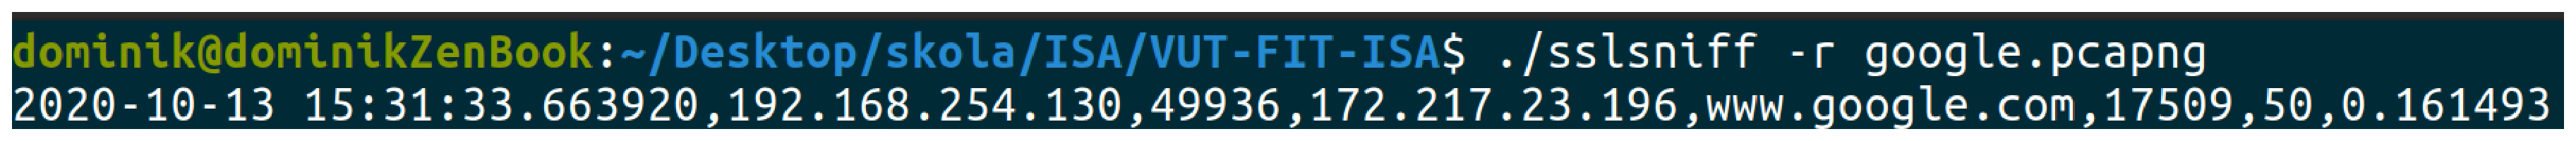
\includegraphics{googleMine.eps}}
	\centering
	\caption{Pcapng súbor spracovaný pomocou sslsniff}
	\end{figure}
	\begin{figure}[h]
	\scalebox{0.17}{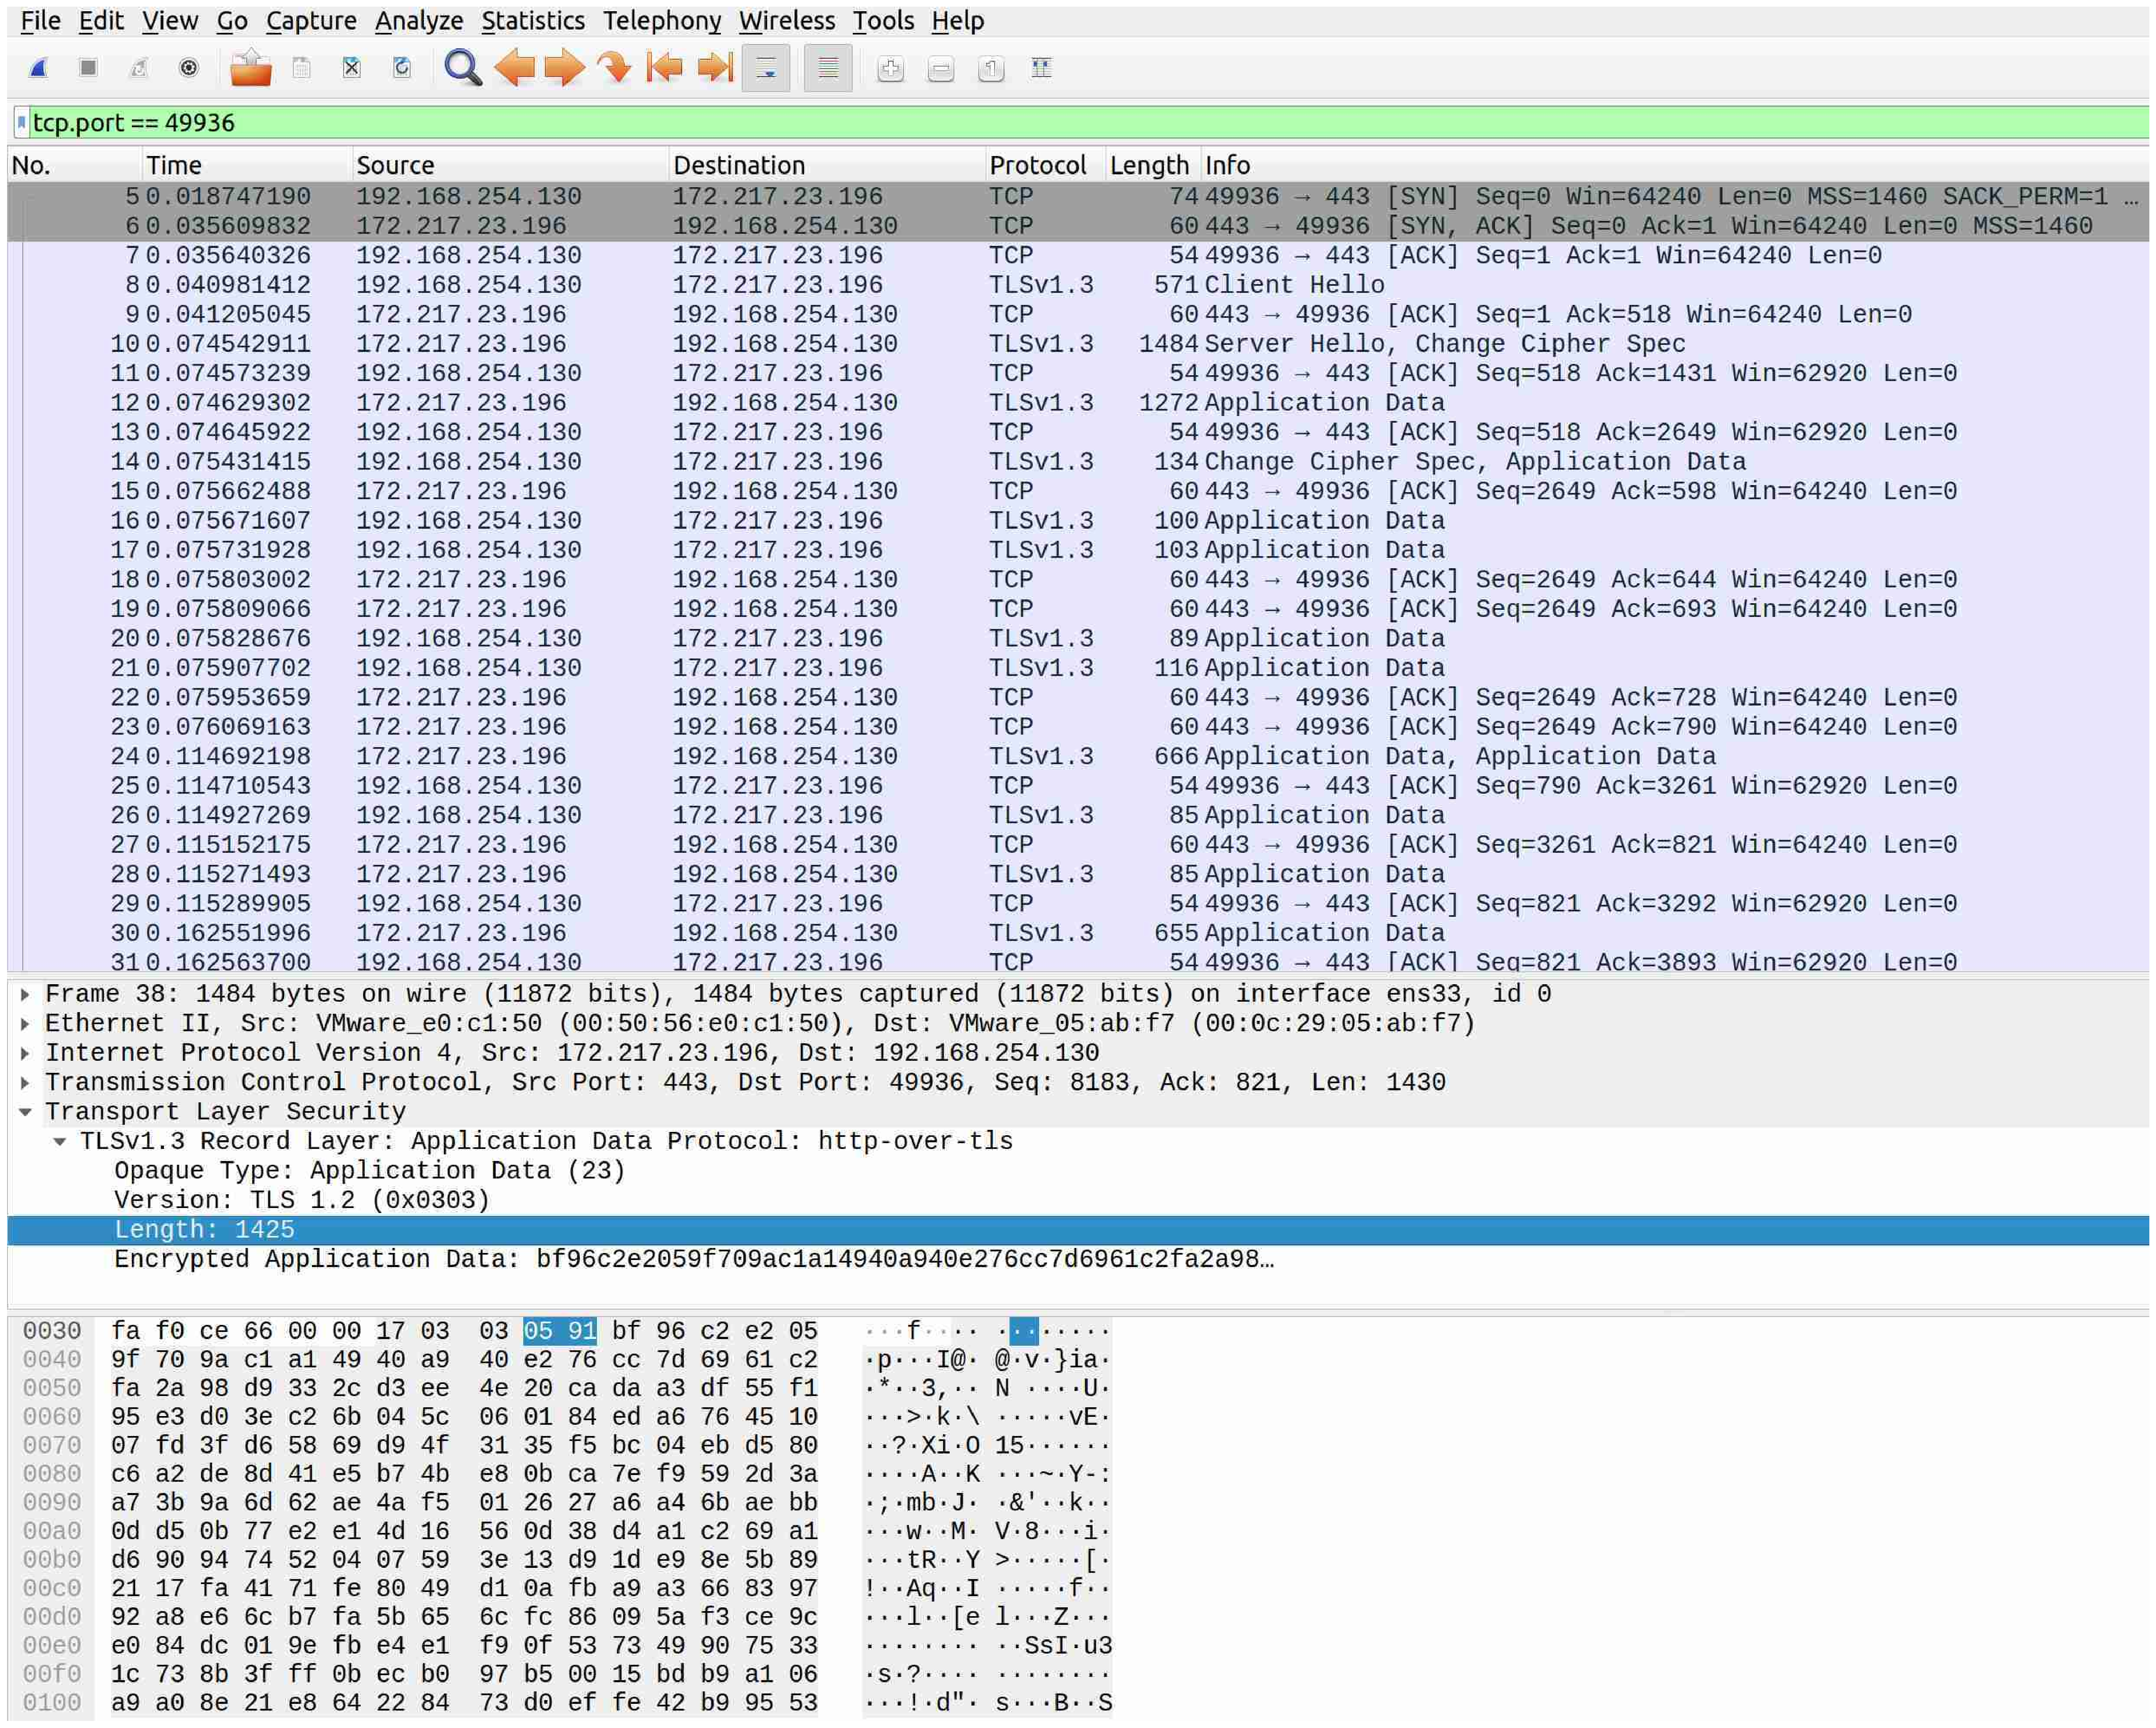
\includegraphics{googleWireshark.eps}}
	\centering
	\caption{Pcapng súbor spracovaný pomocou programu Wireshark}
	
	\end{figure}

	\newpage
	\section{Použité zdroje}
	
	\bibliographystyle{czechiso}
	\renewcommand{\refname}{Použitá literatúra}
	\bibliography{manual.bib}
	
	
\end{document}

	
	
	
